This is obtained by using Google Translate on the original paper written in Korean.


\subsection*{Abstract}

This study conducted a benchmark test using COMSOL Multiphysics, a commercial finite-element-based software widely employed in recent computational geodynamics research. The benchmark involved modeling simple mantle convection while accounting for both incompressible and compressible mantle behavior. The governing equations utilized included the anelastic liquid approximation, truncated anelastic liquid approximation, extended Boussinesq approximation, and Boussinesq approximation; the converged solutions obtained for varying Rayleigh and dissipation numbers were compared. COMSOL Multiphysics proved highly useful for this study due to its user-friendly interface—allowing even non-experts in computational geodynamics to easily construct and run models—and the flexibility it offers for modifying material properties and governing equations. The results align well with established benchmark data. Given its combination of ease of use and accuracy, COMSOL Multiphysics is expected to see widespread application in future computational geodynamics research.


\subsection{Introduction}

If one were to single out the most significant discovery in the history of 20th-century science and engineering, it would be the advent of the computer. 
Since the development of ENIAC (Electronic Numerical Integrator And Computer) (Goldstine, 1972), the first general-purpose computer for ballistic calculations, computer technology has advanced significantly, and currently, computers in almost all fields of science and engineering...
Computers are widely used today. In particular, by enabling massive computational tasks that were previously impossible, computers have driven groundbreaking advancements in the field of numerical analysis; this has made it possible to find numerical solutions for complex partial differential equations that generally lack analytical solutions. Furthermore, the recent emergence of supercomputers—offering vastly superior computational power—has enabled large-scale calculations that were unimaginable just two decades ago.

Consequently, significant efforts have been made since the latter half of the 20th century to solve complex problems in science and engineering using computers and numerical analysis; the geological sciences are no exception to this trend. Even in the 1960s, when computers themselves were a novelty, numerical modeling was employed in pioneering geological research (e.g., McKenzie and Sclater, 1968; Oxburgh and Turcotte, 1968). As computers became more affordable and widely available, research in the geological sciences utilizing computers and numerical analysis expanded rapidly. Within this context, computational geodynamics—a field that uses computers and numerical analysis to study plate motion, deformation, and mantle convection—has established itself as a key area of geological research in the United States, Japan, and advanced European nations. Research in computational geodynamics, covering topics such as mantle convection and subduction processes, continues to be actively conducted today (Sleep, 2006 and references therein; Billen, 2008).


However, computational geodynamics research is an interdisciplinary field that requires knowledge from various related disciplines. First, knowledge of computer programming languages such as Fortran or C is necessary, as well as mathematical knowledge essential for numerical analysis, such as linear algebra and differential equations. Furthermore, because the rheology governing the behavior of plates and the mantle depends on temperature, pressure, and chemical composition, knowledge of geological science and materials science is also required. Due to these characteristics, even developing and utilizing the programs necessary for computational geodynamics research requires significant effort and time; consequently, this acts as an obstacle for geological science majors in acquiring diverse knowledge while conducting research. To overcome this, geological science communities in developed countries [are utilizing specialized computer programmers, applied mathematicians, and geological scientists] with specific characteristics

We have organized a standardized research group and are striving to develop computational geodynamics programs and conduct research using them (e.g., Computational Infrastructure for Geodynamics, www.geodynamic.org and Earthbyte Group, www.earthbyte.org).

Unlike other nations, computational geodynamics research in Korea is still in its infancy; there is a complete lack of comprehensive research programs—such as those found in advanced nations—that utilize specialized research groups to develop and employ relevant software. Therefore, the first priority is to actively introduce geoscientific research utilizing computational geodynamics to the domestic geoscience community and broaden its scope. However, given the critical shortage of researchers in this field, even the initial stage of planning such research—which demands significant time and effort from multiple experts—poses a challenge. Consequently, it is of utmost urgency to foster an environment where not only specialists but also non-specialists can conveniently plan and conduct research, thereby raising awareness and expanding the field's reach.

Given this context, I propose using COMSOL Multiphysics®—a commercial numerical analysis software based on the Finite Element Method (FEM) developed by COMSOL (www.comsol.com)—as an alternative approach for conducting computational geodynamics research. COMSOL Multiphysics is widely utilized across science and engineering fields, enabling the quantitative analysis of complex behaviors in gases, fluids, and solids across one, two, and three dimensions. Notably, it features a Graphical User Interface (GUI) that allows users to easily construct and analyze models using a standard desktop setup with a mouse and keyboard. Furthermore, the software supports parallel computing on supercomputers for computationally intensive tasks, thereby facilitating the execution of highly sophisticated and complex numerical models. In fact, COMSOL Multiphysics has already been frequently employed in studies of plate tectonic processes—such as subduction and mid-ocean ridge dynamics—demonstrating its significant potential for computational geodynamics research (e.g., Carminati and Petricca, 2010; Montési et al., 2011).

Before embarking on full-scale computational geodynamics research using COMSOL Multiphysics—which offers such high potential for application—I intend to conduct the fundamental benchmark tests. While benchmarking of COMSOL Multiphysics for subduction zone modeling has already been performed (van Keken et al., 2008), benchmarks accounting for mantle compressibility and viscous dissipation have not yet been reported. Therefore, in this study, I aimed to compare experimental results obtained using COMSOL Multiphysics with findings from previous studies on 2D incompressible and compressible mantle convection models (King et al., 2010).

%-----------------------------------------------------------------
%-----------------------------------------------------------------
\subsection{Experimental methods}

\subsubsection{2.1: COMSOL Multiphysics}

COMSOL Multiphysics is commercial software based on the finite element method, introduced in 1998 by the Swedish company COMSOL (www.comsol.com), which was founded in 1996; as of December 2012, version 4.3a has been released. It supports the implementation of various 1D, 2D, and 3D numerical models via a graphical user interface, enabling the easy execution of diverse numerical analyses required in science and engineering—ranging from electrical, mechanical, fluid, combustion, and structural analysis to chemical reactions. The program comes with a variety of built-in modeling examples that users can modify to suit their specific needs. Additionally, since material properties can be input as constants or variables, it is possible to construct numerical models with a wide range of material characteristics.

While the modeling examples included in COMSOL Multiphysics are extensive and useful, another significant advantage is the ability for users to freely incorporate ordinary and partial differential equations into their models to suit their specific objectives. This flexibility enables the creation of numerical models tailored to the user's needs. Furthermore, since the built-in differential equations can be modified using simple mathematical notation, anyone with a basic understanding of mathematics can insert or edit these equations.

COMSOL Multiphysics provides post-processing capabilities for results derived from numerical modeling, enabling analysis without the need for external software. For instance, in fluid behavior models, critical parameters such as temperature, pressure, and velocity can be visualized graphically, and specific numerical values can be exported to external files. Furthermore, line, surface, and volume integrals allow for the convenient calculation of various engineering quantities, including fluid and heat flux, enthalpy, and total energy. These features proved particularly useful for comparing the results of this study with those from established benchmarks. More detailed information on COMSOL Multiphysics can be found in the software's manual or in published reference books (e.g., Pryor, 2012).

%-----------------------------------------------------------------
\subsubsection{2.2 Governing Equations for Incompressible and Compressible Mantle Convection}

%-----------------------------------------------------------------
\paragraph{2.2.1 Governing Equations for Mantle Behavior}

Since the establishment of plate tectonics, subduction and mid-ocean ridge spreading can be explained by the global thermochemical circulation occurring between the overriding oceanic plate and the underlying mantle. Mantle behavior, which constitutes the primary component of this thermochemical circulation, can be approximated as the behavior of a highly viscous fluid with temperature- and pressure-dependent viscosity (Schubert et al., 2001). The behavior of such a highly viscous fluid can be described as compressible laminar flow; the governing equations for this flow—partial differential equations representing the conservation of mass, momentum, and energy—are expressed as the continuity, momentum, and energy equations, respectively, as follows (Schubert et al., 2001).

\begin{center}
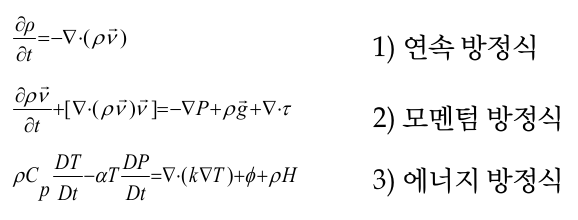
\includegraphics[width=8cm]{images/lee_13/eq_123}
\end{center}

Here, $\rho$ is density (kg/m³), $t$ is time (s), $v$ is the velocity vector (m/s), 
$P$ is pressure (Pa), $g$ is the gravitational acceleration vector (m/s²), 
$\tau$ is the deviatoric stress tensor (Pa), $C_p$ is the isobaric heat capacity (J/kg·K), 
$T$ is temperature (K), $\alpha$ is the thermal expansion coefficient (/K), 
$k$ is thermal conductivity (J/m·K·s), $\phi$ is viscous dissipation per unit volume (J/m³·s), 
and i$H$ is the rate of internal thermal energy generation per unit mass (J/kg·s). 
Viscous dissipation represents the amount of fluid momentum converted into thermal energy i
due to shear stresses arising from fluid motion and is defined as follows.

\begin{center}
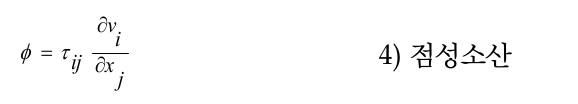
\includegraphics[width=8cm]{images/lee_13/eq_4}
\end{center}

If the mantle were chemically homogeneous and lacked dynamic behavior (such as convection), its density could be expressed solely as a function of temperature and pressure; this is defined as the "reference state." Mantle dynamics—specifically convection—arise from spatial density variations, which are caused by deviations in temperature and pressure from the reference state. Therefore, the actual density of the mantle can be represented by the linear sum of the density defined by the reference state and the density difference resulting from deviations in temperature and pressure. This relationship is expressed mathematically as follows.

\begin{center}
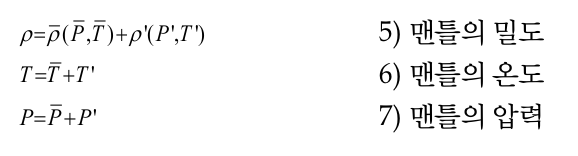
\includegraphics[width=8cm]{images/lee_13/eq_567}
\end{center}

In the above equation, $\rho$, $T$, and $P$ represent the density, temperature, and pressure 
corresponding to the reference state, respectively, while $\rho'$, $T'$, and $P'$ 
represent the density, temperature, and pressure deviating from the reference state. 
In the absence of mantle flow, the reference-state density can be described by the 
Adams-Williamson equation of state (Birch, 1952).


\begin{center}
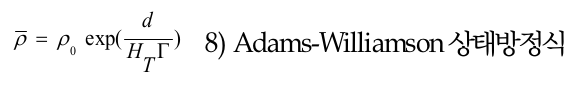
\includegraphics[width=8cm]{images/lee_13/eq_8}
\end{center}

$\rho_0$ is the density of the mantle at the surface, HT is the temperature 
scale height of the compressible fluid, and $\Gamma$ is the Grüneisen parameter; they are defined as follows:

\begin{center}
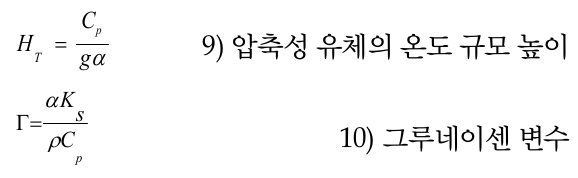
\includegraphics[width=8cm]{images/lee_13/eq_910}
\end{center}

Ks represents the isentropic bulk modulus. By substituting the variables—mantle density, temperature, and pressure—into the governing equation presented above, one can calculate the behavior of the mantle; the following section describes various approximate equations for mantle behavior derived from that governing equation.

%-----------------------------------------------------------------
\paragraph{2.2.2 Anelastic Liquid Approximation (ALA)}

The governing equations for mantle behavior can be simplified because the mantle satisfies the following assumptions (Schubert et al., 2001). First, since the variation in mantle density is negligible compared to the mantle's velocity, the left-hand side of the continuity equation can be approximated as zero. Second, because mantle acceleration is extremely low, the mantle behaves as a fluid with a Mach number effectively equal to zero and a very high Prandtl number (exceeding 10²²). Consequently, the left-hand side of the momentum equation can also be approximated as zero. Applying these two assumptions to the governing equations yields the following set of equations, known as the anelastic liquid approximation (ALA).

\begin{center}
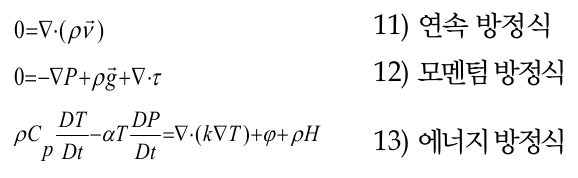
\includegraphics[width=8cm]{images/lee_13/eq_111213}
\end{center}

To efficiently compute the governing equations, non-dimensionalization is performed using the following relevant expressions.

\begin{center}
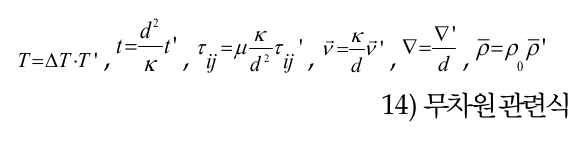
\includegraphics[width=8cm]{images/lee_13/eq_14}
\end{center}

$\Delta T$ is the temperature difference between the top and bottom surfaces of the mantle, 
$d$ is the mantle thickness (m), $\kappa$ is the thermal diffusivity (m²/s), 
$\mu$ is the dynamic viscosity (Pa·s), and $\rho_0$ is the density at the mantle surface (kg/m³). 
After non-dimensionalization, the governing equations-written without the prime symbol for 
convenience-are as follows:

\begin{center}
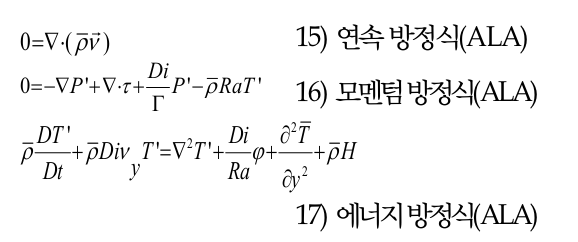
\includegraphics[width=8cm]{images/lee_13/eq_151617}
\end{center}

Non-dimensionalization leads to the derivation of the dissipation number (Di) and the Rayleigh number (Ra), which are defined as follows:

\begin{center}
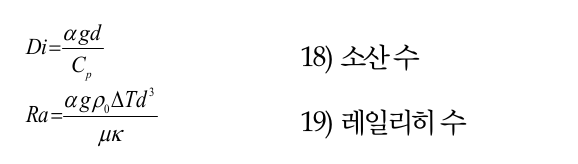
\includegraphics[width=8cm]{images/lee_13/eq_1819}
\end{center}

Since non-dimensionalization also applies to the reference state equation for density, the reference state equation is redefined as follows.

\begin{center}
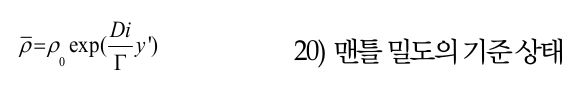
\includegraphics[width=8cm]{images/lee_13/eq_20}
\end{center}

The variable y' represents the mantle depth normalized by the mantle thickness, taking a value of 0 at the surface and 1 at the base. This reference state equation indicates that mantle density increases linearly with depth. The increase in mantle density can be approximated as resulting from adiabatic compression, and the reference state equation for the temperature rise caused by adiabatic compression is derived as follows.

\begin{center}
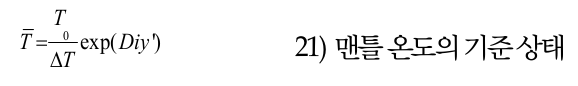
\includegraphics[width=8cm]{images/lee_13/eq_21}
\end{center}

T0 is the temperature at the mantle surface. Like density, this equation indicates that the mantle temperature increases with depth due to adiabatic compression.

%-----------------------------------------------------------------
\paragraph{2.2.3 Truncated Anelastic Liquid Approximation, TALA}


For some numerical modeling packages, difficulties arise in incorporating the dynamic pressure term into the momentum equation due to technical issues (King et al., 2010). In such cases, the dynamic pressure term $\nabla P'$ is omitted from the momentum equation of the anelastic liquid approximation, resulting in the use of the truncated anelastic liquid approximation (TALA). The remaining equations are identical to those of the anelastic liquid approximation.

\begin{center}
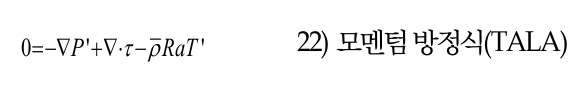
\includegraphics[width=8cm]{images/lee_13/eq_22}
\end{center}

%-----------------------------------------------------------------
\paragraph{2.2.4 (Extended Boussinesq Approximation, EBA)}

The extended Boussinesq approximation (EBA) is an approximation reformulated from the truncated inelastic fluid approximation by assuming the reference-state density to be constant; its governing equations are defined as follows:

\begin{center}
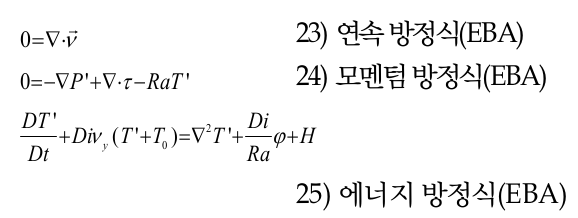
\includegraphics[width=8cm]{images/lee_13/eq_232425}
\end{center}

Vy is the velocity vector in the y-direction. This governing equation is useful for approximating mantle behavior at relatively shallow depths, where the effect of density increase with depth is not significant.



%-----------------------------------------------------------------
\paragraph{2.2.5 (Boussinesq Approximation, BA)}



The Boussinesq Approximation (BA) represents the most simplified governing equations describing the behavior of an incompressible fluid. This approximation is derived by assuming a dissipation number of zero in the energy equation of the extended Boussinesq approximation. Consequently, this assumption is suitable for modeling mantle behavior—where heat generation due to viscous dissipation is expected to be negligible—and is formulated as follows.

insert eq 26

Further details regarding the governing equations described above can be found in previous studies (Jarvis and McKenzie, 1980; Schubert et al., 2001; King et al., 2010). As previously mentioned, the anelastic fluid approximation is the governing equation that most accurately represents mantle behavior. However, due to factors such as technical limitations or the need for model simplification, models employing simplified governing equations—such as the Boussinesq approximation—remain widely used.



%-----------------------------------------------------------------
\paragraph{2.3 Numerical Model}


The derived governing equations and the reference state equations were implemented in COMSOL Multiphysics, and a benchmark study was conducted using two-dimensional finite element modeling. The model used for the benchmark is based on the one presented by King et al. (2010) and is summarized as follows. The model domain is a two-dimensional square; the top and bottom walls are fixed at temperatures of 273 K and 3273 K, respectively, while the side walls are insulated. Additionally, a free-slip condition is assumed for the stress state at all walls, implying that no shear stress acts on the fluid flow. Mantle convection is driven by the temperature difference (3000 K) between the top and bottom walls.
Since the governing equations employed in this study utilize dimensionless quantities, all values used in the modeling are dimensionless. Although mantle viscosity varies significantly depending on temperature, pressure, and composition (Karato and Wu, 1993; Ranalli, 2001), it was assumed to be constant for the sake of the benchmark. Additionally, while internal thermal energy is generated within the mantle through the decay of radioactive isotopes, this factor was neglected for the benchmark (H = 0). The coefficients and constants used in the modeling are listed in Table 1.


In numerical analysis using the finite element method, the accuracy of calculations is significantly affected by the efficiency of mesh formation that constitutes the modeling scope. Generally, using more elements leads to higher accuracy, but this is inefficient because the computation time required for modeling increases significantly as the number of elements increases. COMSOL Multiphysics fundamentally supports the formation of meshes composed of various elements, such as triangles and quadrilaterals.

In this study, a user-controlled mesh was used, and the mesh size was configured to homogeneously form the entire domain using triangular elements suitable for fluid dynamics modeling provided by COMSOL Multiphysics.

Mesh refinement was based on the convection measured at the upper wall of the domain

Mesh refinement is necessary to more accurately measure the Nusselt number—defined as the ratio of convective to conductive heat energy loss at the upper wall of the domain—and the convective velocity at that wall. To achieve this, the upper section of the domain was composed of smaller mesh elements through a three-stage refinement process (Figure 1). The total number of elements resulting from this refinement is 16,065.

For the numerical modeling, the Rayleigh number—a parameter used in previous studies—was varied across the values 
of $10^4$, $2\times 10^4$, $5\times 10^4$, $10^5$, $2\times 10^5$, $5\times 10^5$, and $10^6$. 
Separate experiments were conducted for each Rayleigh number using dissipation numbers of 0.25, 0.50, 1.0, 1.5, and 2.0. When a dissipation number is present, a corresponding reference state equation for mantle temperature—determined by adiabatic compression—exists for each specific dissipation number. For benchmarking purposes in this study, the reference state equation was linearly added to the mantle temperature such that the value at the base of the mantle equaled 3273 K (dimensionless value: 1). In other words, the net temperature difference driving mantle behavior is defined as the total mantle temperature minus the reference state value.


In experiments employing the Boussinesq approximation, terms related to the dissipation number are absent; therefore, the experiments were conducted by varying only the Rayleigh number. A time-dependent solver was used to perform calculations up to a dimensionless time of 1.0, allowing the system to reach a steady state where the results effectively converged. Typically, to initiate mantle convection, COMSOL Multiphysics applies an internal temperature perturbation as an initial condition, which generally results in the formation of a single convection cell within the modeling domain. However, in experiments with high Rayleigh and dissipation numbers, the system may converge to a state with two or more convection cells rather than a single cell. To encourage convergence toward a single convection cell, some experiments utilized the temperature distribution calculated at a lower Rayleigh number as the initial temperature distribution—a method also employed in previous benchmark studies (King et al., 2010).

%------------------------------------
\subsection{Experimental Results}



\subsubsection{3.1 Benchmark}

\paragraph{3.1.1 Anelastic fluid approximation}

First, let us examine the results obtained by varying the Rayleigh number and the dissipation number in a benchmark 
study conducted using the governing equations of the anelastic fluid approximation. Table 2 presents the benchmark 
results, including the Nusselt number (Nu), the maximum velocity at the upper surface of the convecting mantle (Vsurf-max), 
the line integral value of velocity at the upper surface (Vsurf), the average temperature of the entire convection 
cell ($\langle T \rangle$), the thermal energy generated by viscous dissipation within the cell ($\langle \phi \rangle$), 
and the work done by the mantle against gravity ($\langle W \rangle$). Note that all values presented here are 
dimensionless. For details on the calculation methods for these values, please refer to the existing benchmark 
study used for comparison in this research (King et al., 2010).

It was confirmed across all experiments --regardless of the dissipation number-- that the intensity of convection increases 
as the Rayleigh number rises (Figure 2; Table 2). The fact that convective intensity increases with the Rayleigh number 
is already well established (e.g., Blankenbach et al., 1989; King et al., 2010). Figure 2 illustrates the 
temperature distribution within convection cells as the Rayleigh number increases by an order of magnitude --from $10^4$ 
to $10^5$ and then to $10^6$-- while the dissipation number remains fixed at 0.25.


As is already known, it is observed that the thickness of the thermal boundary layers at the top and bottom of 
the convection cells decreases as the Rayleigh number increases; this is reflected in the increase of the Nusselt 
number (Nusselt numbers of 4.410, 9.229, and 14.867 correspond to experimental results obtained with Rayleigh numbers 
of $10^4$, $10^5$, and $10^6$, respectively).
As the intensity of convection increases, the mantle convection velocity rises; this is clearly reflected in the 
increase of both the maximum convection velocity at the upper surface and the line integral value alongside the 
rise in the Rayleigh number (specifically, $V_{surf-max}$ values of 58.065, 252.509, and 749.419 correspond to experiments 
using Rayleigh numbers of $10^4$, $10^5$, and $10^6$, respectively, while $V_{surf}$ values of 38.826, 184.406, 
and 540.730 correspond to the same Rayleigh numbers). Thermal energy due to viscous dissipation ($\langle\phi\rangle$) 
exhibits a linear increase with the Rayleigh number. Similarly, the work done by the mantle against gravity ($\langle W\rangle$) 
shows a linear increase with the Rayleigh number, yielding values nearly identical to those of the thermal energy 
from viscous dissipation. Jarvis and McKenzie (1980) demonstrated that the thermal energy from viscous dissipation and 
the work done by the mantle against gravity exactly cancel each other out; the results of this study confirm that 
these two quantities effectively cancel each other out as well. Furthermore, the mesh resolution test presented 
later in this paper (Section 3.2) indicates that the errors observed in this experiment stem from mesh resolution rather than from any flaws in the governing equations.

Unlike the intensity of convection, which increases with the Rayleigh number, an increase in the dissipation number weakens convective 
intensity (Figure 3). This is clearly demonstrated by the decrease in the benchmark result values as the dissipation number rises. For 
instance, at a dissipation number of 2.0, convective intensity weakens drastically; at a Rayleigh number of $10^4$, 
only very weak convection is observed. A Nusselt number approaching 1 indicates that heat transfer within the mantle 
occurs almost exclusively via conduction rather than convection (at a Nusselt number of 1, mantle convection does not 
occur, and heat transfer relies solely on conduction). This indicates that, unlike the Rayleigh number—which is positively 
correlated with convective intensity—the dissipation number shares an inverse relationship with it.

The results obtained in this experiment were compared with existing benchmark results. With few exceptions, the results showed good agreement with established benchmarks; notably, they aligned very closely—within a relative error of 1\%—with the results from the Virginia Tech (VT) study (King et al., 2010) that utilized the ConMan program (King et al., 1990). Furthermore, for the experiment involving the development of two convection cells, the results showed good agreement with those from the University of Colorado (CU) study that used the Citcom program (Moresi et al., 1996). Although the relative error was observed to increase slightly in experiments with high dissipation numbers, it remained low, generally falling within the 1-4\% range.




\paragraph{3.1.2 Truncated Anelastic Fluid Approximation}
This section summarizes the experimental results obtained using the truncated anelastic approximation governing equations. The truncated anelastic approximation is derived by omitting only the dynamic pressure term from the momentum equation of the standard anelastic approximation. It is generally understood that the dynamic pressure term has a relatively minor influence on fluid behavior compared to other terms (King et al., 2010).

To quantitatively evaluate the impact, results obtained using the governing equations for the truncated anelastic fluid approximation were compared with those obtained using the governing equations for the anelastic fluid approximation. As shown in Figure 4, which plots the relative errors of the comparable results, the discrepancy caused by the dynamic pressure term is relatively large at low Rayleigh numbers. However, the relative error tends to decrease as the Rayleigh number increases. This reduction in relative error—observed in the Nusselt number, thermal energy from viscous dissipation, and work done by the mantle against gravity—is particularly pronounced as the Rayleigh number rises; at Rayleigh numbers of $5 \times 10^5$ or higher, the relative error becomes very small, falling within 2\%. Given that the Rayleigh number of the Earth's mantle is estimated to be around $10^6$ (Schubert et al., 2001), these results indicate that the governing equations for the truncated anelastic fluid approximation can effectively approximate those for the anelastic fluid approximation.

As observed in Table 3, the relative error between the thermal energy generated by viscous dissipation and the work done by the mantle against gravity generally falls within the 0.1–6\% range. When compared with existing experimental results (King et al., 2010), the relative error showed a tendency to increase in experiments with high dissipation numbers but remained low--mostly around 1–4\%--in most cases; significant relative errors of 8–13\% were observed only in experiments using a dissipation number of 2.0 and a low Rayleigh number (e.g., Rayleigh number of $10^4$). 
Overall, however, the experimental results of this study were found to be consistent with those of existing benchmarks.

\paragraph{3.1.3 Extended Boussinesq Approximation}


The extended Boussinesq approximation incorporates the assumption of mantle incompressibility into the truncated anelastic fluid approximation; consequently, the adiabatic temperature profile resulting from adiabatic compression is absent. Due to this assumption, a common approach—used to approximate the actual temperature structure where adiabatic compression occurs—involves conducting experiments based on potential temperature and then linearly adding the adiabatic temperature profile to the results (e.g., Billen and Hirth, 2007; Lee and King, 2011). However, as the primary objective of this study is to benchmark the COMSOL Multiphysics software, no direct comparison regarding these differences was conducted. Therefore, the results obtained using the extended Boussinesq governing equations were not directly compared with the previously described experimental results.

However, the effects of the Rayleigh number and the dissipation number on mantle convection are similar to the experimental results mentioned earlier. The intensity of mantle convection increases as the Rayleigh number rises, whereas it decreases as the dissipation number increases (Table 4). Notably, when the dissipation number is 2.0, mantle convection does not occur in experiments using Rayleigh numbers of $10^4$ and $2 \times 10^4$; this represents a case where the inhibiting effect of viscous dissipation on fluid motion is maximized. It is also noteworthy that, under the extended Boussinesq approximation, the discrepancy between the thermal energy generated by viscous dissipation and the work done by the mantle against gravity is minimal—a trend clearly observed even in experiments employing high Rayleigh and dissipation numbers. The experimental results were compared with existing benchmark data, revealing a relative error of less than 1\% in most cases (results for dissipation numbers of 1.5 and 2.0 
were excluded from the comparison as they were not reported in the existing benchmark studies).


\paragraph{3.1.4 Boussinesq Approximation, BA}

Finally, a benchmark study was conducted using the Boussinesq approximation—the most commonly employed set of governing equations for fluid behavior. As shown in Table 5, the Boussinesq approximation produces the most vigorous mantle convection compared to experiments using other approximate governing equations. Furthermore, in contrast to other approximations—where the flow tends to converge into two or three convection cells or exhibit time-dependent behavior as the Rayleigh number increases—the Boussinesq approximation consistently demonstrated stable convergence to a single convection cell, even at high Rayleigh numbers. These experimental results were compared with existing benchmark data, and all showed a relative error of less than 1\%.

\subsubsection{3.2 Mesh Resolution Test}

In addition to benchmarking the various governing equations introduced above, mesh resolution tests were conducted. Specifically, these tests allowed for the verification of whether the thermal energy generated by viscous dissipation and the work done by the mantle against gravity align accurately within the anelastic fluid approximation framework. While the aforementioned experiments achieved more precise Nusselt number measurements by refining the upper mesh region, the resolution tests focused on varying the element size across three levels without specifically refining the upper mesh section. The experiment using the fewest elements employed the "coarse" mesh setting provided by COMSOL Multiphysics, resulting in a total of 578 elements. The "fine" setting utilized 2,124 elements, while the "extra fine" setting—representing the highest resolution—generated a total of 15,244 elements. To facilitate the mesh resolution tests, the dissipation number was fixed at 0.5, and experiments were conducted by varying only the Rayleigh number.

Table 6 presents the results of the resolution tests conducted for each governing equation. In the experiments using the governing equations based on the anelastic fluid approximation, the Nusselt number is observed to increase as the mesh resolution increases. This occurs because the Nusselt number is calculated using elements closest to the upper surface; consequently, smaller element sizes allow for a more accurate measurement of temperature variations within the thermal boundary layer. In other words, a more accurate Nusselt number is obtained when the element size is smaller.

It was observed that while the Nusselt number is significantly affected by mesh resolution, the differences in other result values are relatively minor. This indicates that modeling results for mantle behavior do not vary substantially even when a relatively small number of elements is used. However, since a tendency for error to increase with the Rayleigh number was observed, a certain level of mesh resolution is essential for accurately calculating mantle behavior at Rayleigh numbers around $10^7$.

In experiments using the governing equations for the anelastic fluid approximation, 
it is observed that the discrepancy between the thermal energy generated by viscous 
dissipation and the work done by the mantle against gravity decreases as mesh resolution 
increases, regardless of the Rayleigh number. Notably, with "extra fine" mesh resolution, 
the relative error between these two calculated values remains within 0.001\% across 
all experiments, indicating that the governing equations for the anelastic fluid approximation 
have been accurately implemented in COMSOL Multiphysics. In contrast, for the truncated 
anelastic fluid approximation—in which the dynamic pressure term is omitted from the momentum 
equation—a nearly constant relative error between the thermal energy from viscous dissipation 
and the work done by the mantle against gravity is observed, irrespective of mesh resolution.


In the case of experiments using the extended Boussinesq approximation governing equations, the observation that the relative error between thermal energy (generated by viscous dissipation) and the work done by the mantle against gravity decreases in proportion to the increase in mesh resolution clearly indicates that higher mesh resolution contributes to improved experimental accuracy. In experiments employing the Boussinesq approximation governing equations, viscous dissipation is absent, and—as in other experiments—increasing the mesh resolution significantly contributes to improving the accuracy of the Nusselt number.

\subsection{Discussion and Conclusion}




Benchmarking results for incompressible and compressible mantle convection, obtained using the finite element-based commercial software COMSOL Multiphysics, showed excellent agreement with existing benchmark results. This demonstrates that COMSOL Multiphysics ensures the accuracy and reliability required for mantle convection modeling while offering advantages such as a graphical user interface and the ease of modifying or inserting material properties and governing equations.

Experiments conducted using various governing equations have demonstrated that mantle compressibility significantly influences the mantle's temperature and convective structure. The estimated dissipation number for the mantle is approximately 0.5, and the Rayleigh number is around $10^7$. Figure 5 presents the converged results of mantle convection calculated for each set of governing equations, assuming a dissipation number of 0.5 and a Rayleigh number of $5 \times 10^5$. As clearly shown in the temperature distributions, experiments accounting for compressibility (Figures 5a and 5b) yield similar results to each other but differ significantly from the experiment conducted under the assumption of incompressibility (Figure 5d). Furthermore, even the experiment utilizing the Extended Boussinesq Approximation—which incorporates the incompressibility assumption into the governing equations of the Anelastic Liquid Approximation (Figure 5c)—shows a marked difference in temperature distribution compared to the experiment based on the incompressibility assumption (Figure 5d). This strongly indicates that, in addition to mantle compressibility, viscous dissipation exerts a significant influence on the mantle's temperature and flow structure.

As this study was conducted to benchmark various programs used for mantle convection research, it did not account for the actual physical properties of the mantle or the phase transformations occurring within it. Viscosity, a key factor influencing actual mantle behavior, can be approximated by diffusion and dislocation creep and is significantly affected by temperature, pressure, grain size, and strain rate (Karato and Wu, 1993; Ranalli, 2001). Therefore, it should be noted that this experiment, which assumes constant viscosity, represents a simplified model of actual mantle behavior. Furthermore, phase transformations (such as olivine to wadsleyite) and phase dissociations (such as ringwoodite to perovskite plus magnesiowüstite)—driven by increasing temperature and pressure—can either enhance or inhibit mantle convection processes like subduction and mantle plumes (King and Ita, 1995; Ita and King, 1998). Consequently, the combined effects of these phase changes and dissociations, along with mantle compressibility and viscous dissipation, would collectively influence mantle temperature and dynamics.

Despite the use of simplified and idealized experimental setups, this study demonstrates that COMSOL Multiphysics offers both convenience and accuracy for modeling mantle convection and subduction, holding significant potential to contribute to future research in this field. Most existing studies have investigated mantle convection and subduction using governing equations that assume mantle incompressibility (such as the Boussinesq approximation)—an approach that remains widely used today. Although some studies have made limited comparisons regarding the effects of compressibility on mantle temperature and behavior (Lee and King, 2009), future research on mantle dynamics and subduction processes must consider mantle compressibility as a crucial modeling factor. The benchmark results presented here are encouraging and serve as a promising starting point for future computational geodynamics research.

Acknowledgments

We would like to express our gratitude to Professors Seung-Seop Kim and Young-Hee Kim for their valuable contributions to improving the quality of this paper. We also thank Professor Young-Kwan Sohn, the Editor-in-Chief, for his assistance. This research was supported by the National Research Foundation of Korea (NRF) with funding from the government (Ministry of Education, Science and Technology) in 2011 (NRF-2011-35B-1-C00043).


\begin{center}
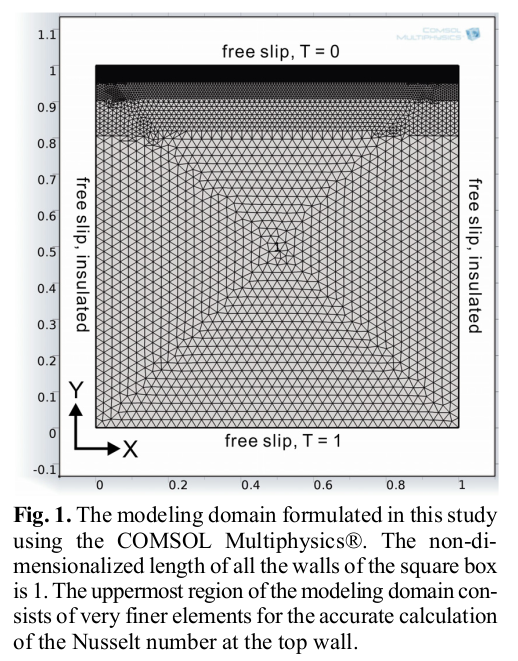
\includegraphics[width=7cm]{images/lee_13/fig1}
\end{center}

\begin{center}
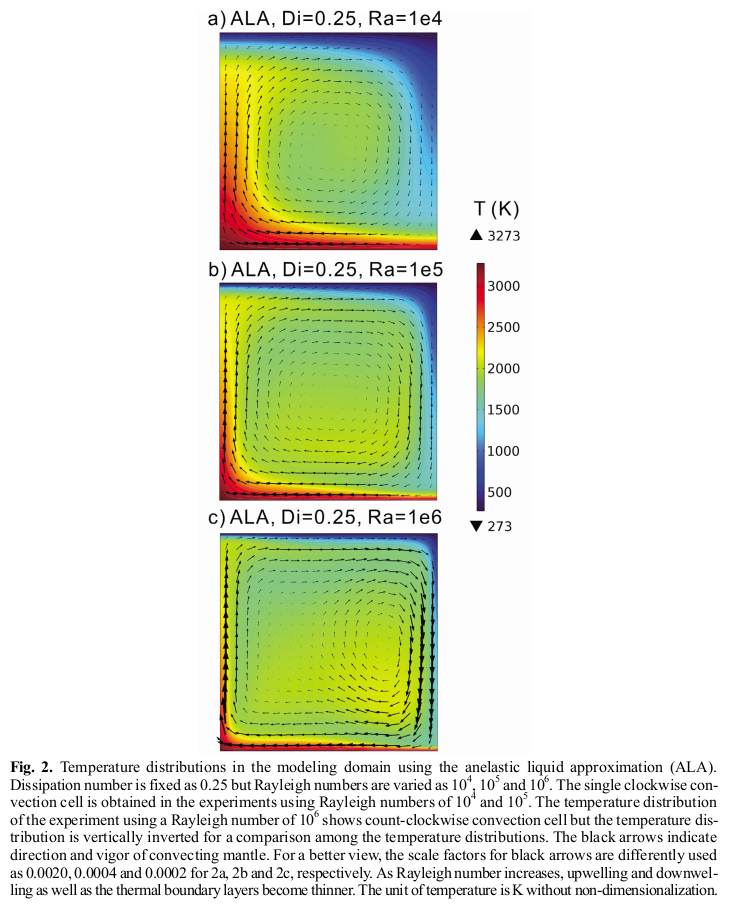
\includegraphics[width=12cm]{images/lee_13/fig2}
\end{center}

\begin{center}
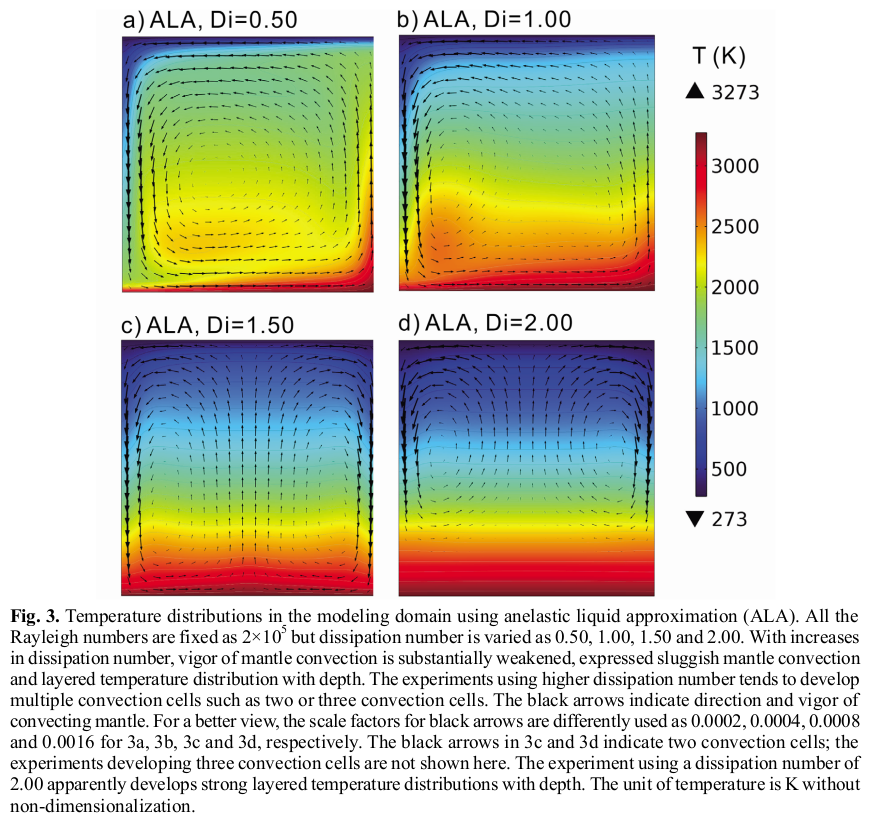
\includegraphics[width=12cm]{images/lee_13/fig3}
\end{center}

\begin{center}
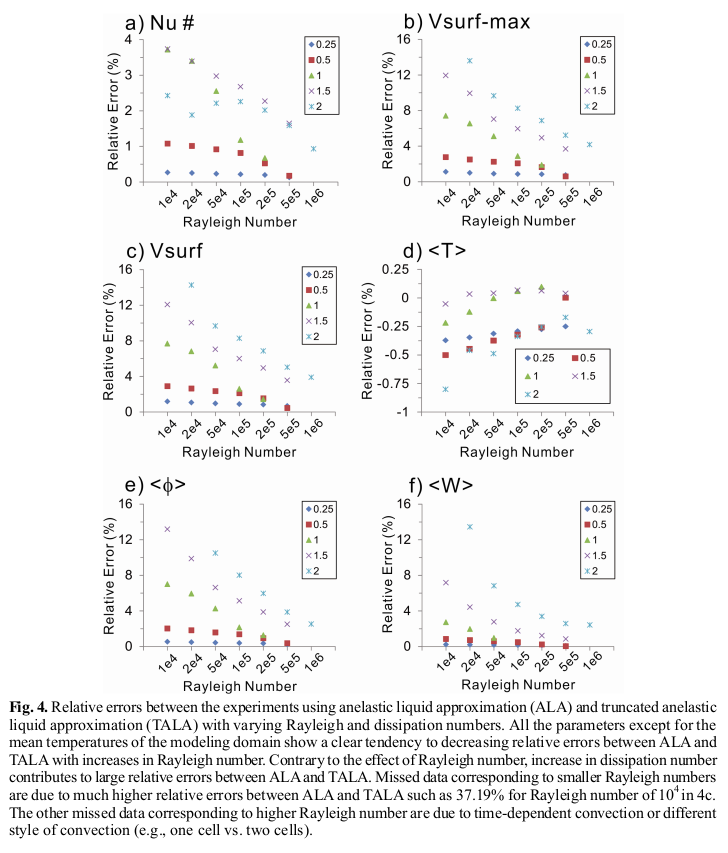
\includegraphics[width=12cm]{images/lee_13/fig4}
\end{center}

\begin{center}
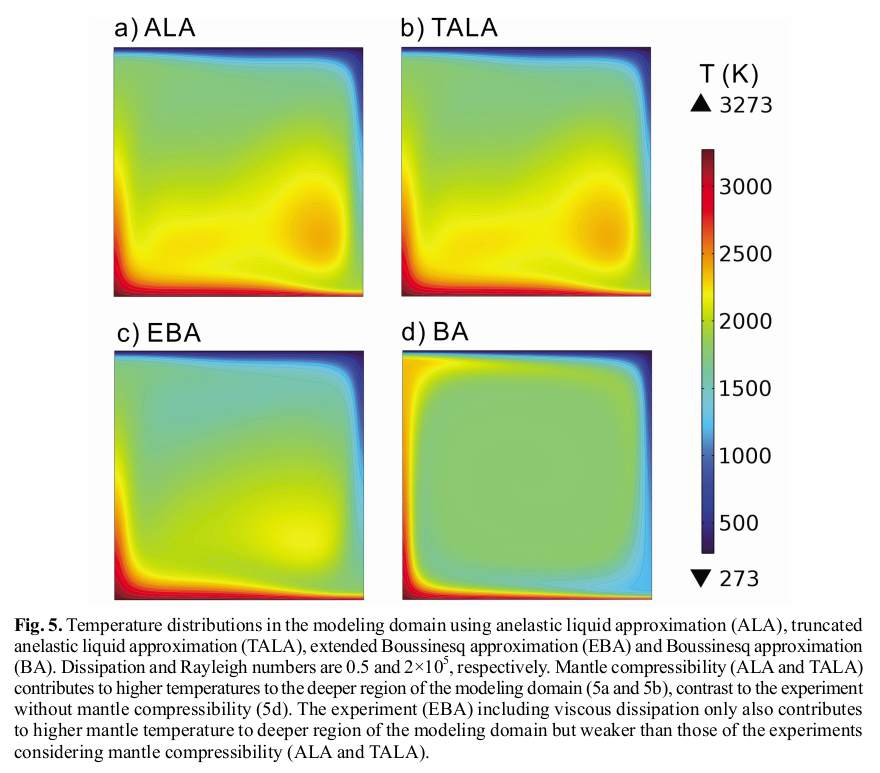
\includegraphics[width=12cm]{images/lee_13/fig5}
\end{center}



\begin{center}
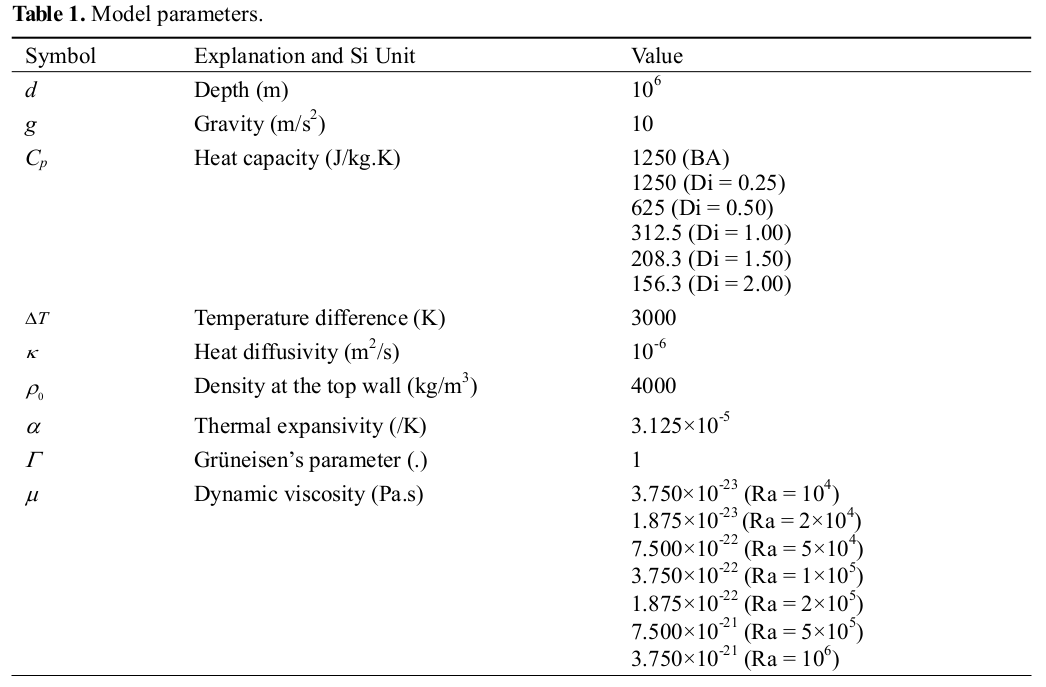
\includegraphics[width=12cm]{images/lee_13/table1}
\end{center}

\begin{center}
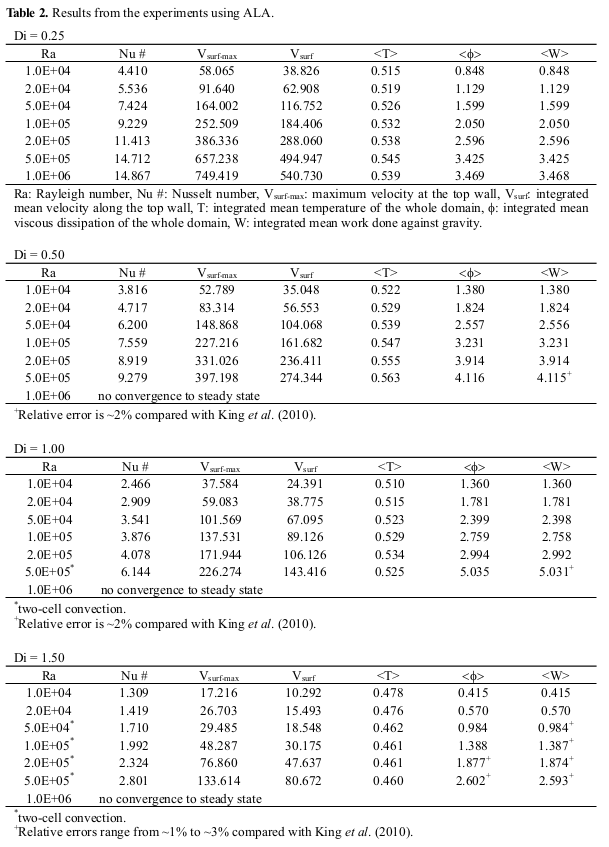
\includegraphics[width=12cm]{images/lee_13/table2a}
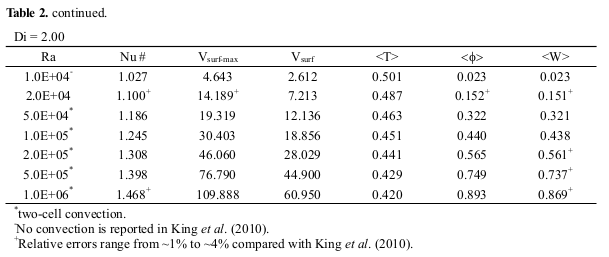
\includegraphics[width=12cm]{images/lee_13/table2b}
\end{center}

\begin{center}
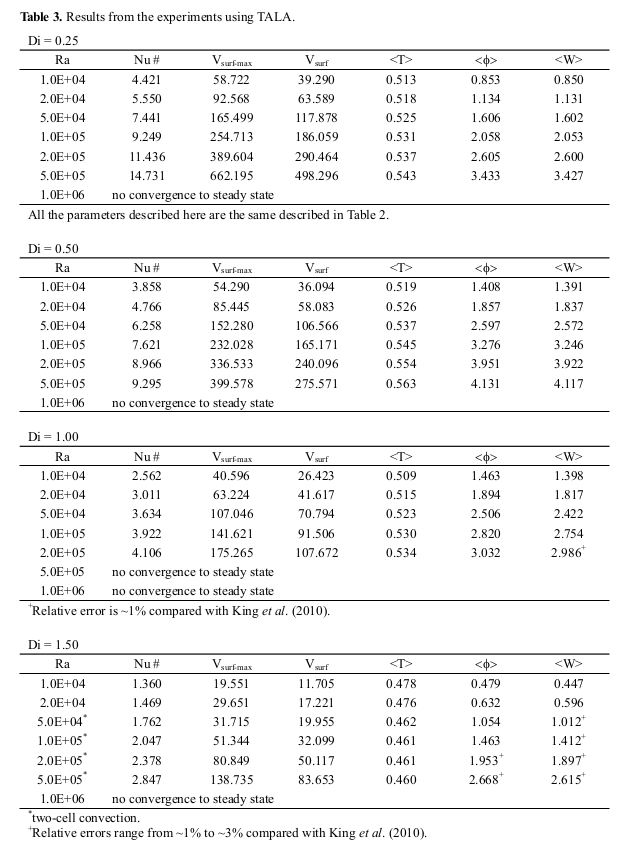
\includegraphics[width=12cm]{images/lee_13/table3a}
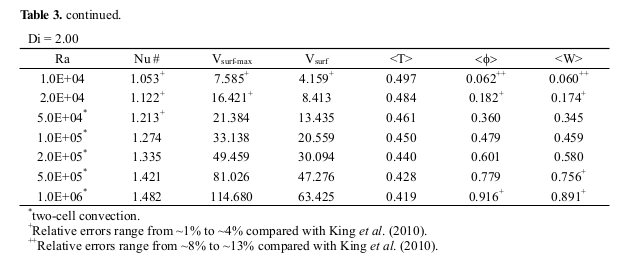
\includegraphics[width=12cm]{images/lee_13/table3b}
\end{center}

\begin{center}
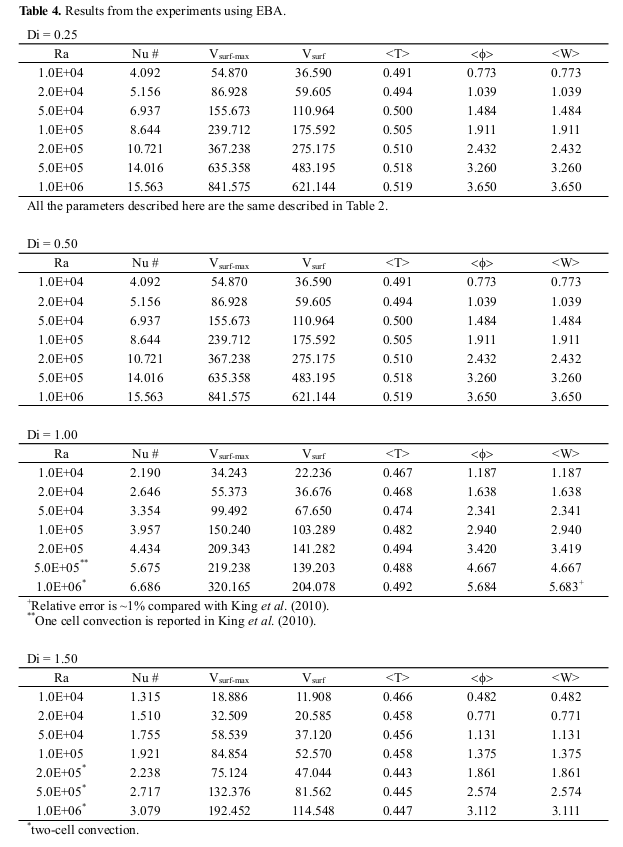
\includegraphics[width=12cm]{images/lee_13/table4a}
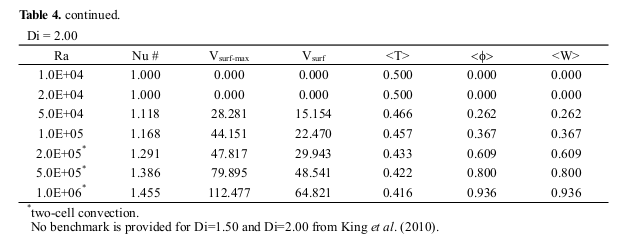
\includegraphics[width=12cm]{images/lee_13/table4b}
\end{center}

\begin{center}
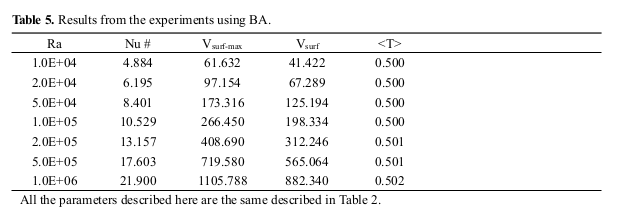
\includegraphics[width=12cm]{images/lee_13/table5}
\end{center}

\begin{center}
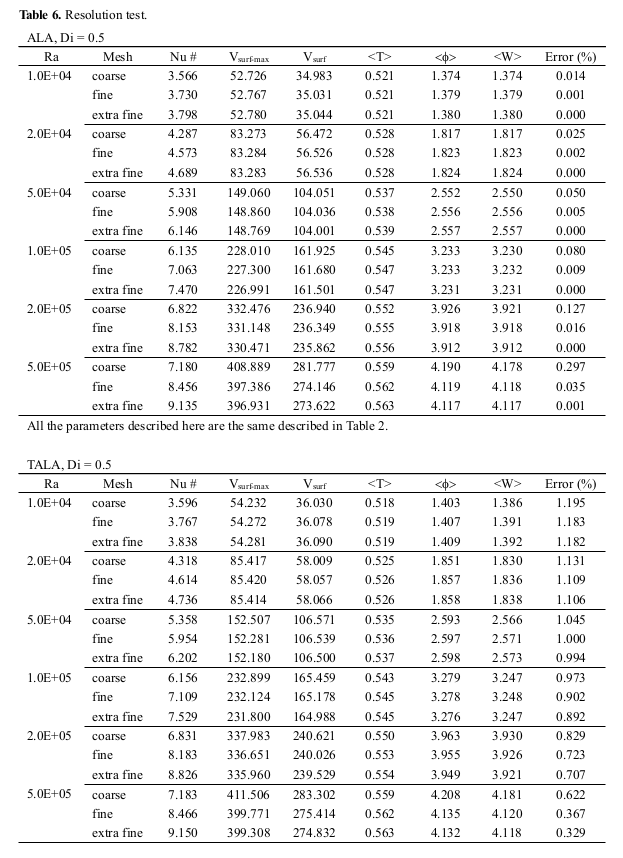
\includegraphics[width=12cm]{images/lee_13/table6a}
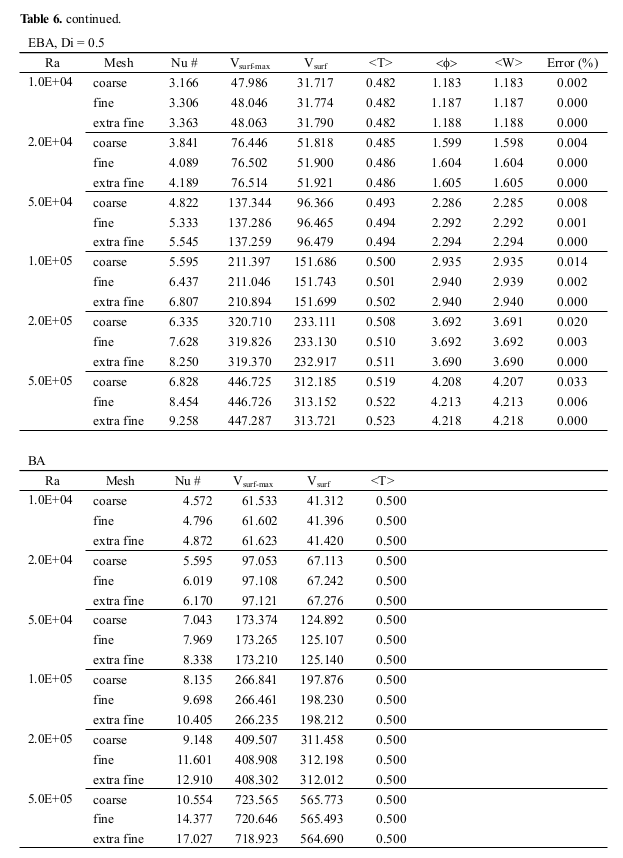
\includegraphics[width=12cm]{images/lee_13/table6b}
\end{center}






















